% !TEX program = xelatex
\documentclass[degree=undergraduate,bibstyle=numerical,font=empty]{xmuthesis}

\usepackage{geometry}
\geometry{a4paper,scale=0.8}

\DeclareMathOperator*{\argmin}{argmin}

\usepackage{paralist}

\usepackage{rotating}

\makeatletter
\newenvironment{breakablealgorithm}
  {% \begin{breakablealgorithm}
   \begin{center}
     \refstepcounter{algorithm}% New algorithm
     \hrule height.8pt depth0pt \kern2pt% \@fs@pre for \@fs@ruled
     \renewcommand{\caption}[2][\relax]{% Make a new \caption
       {\raggedright\textbf{\fname@algorithm~\thealgorithm} ##2\par}%
       \ifx\relax##1\relax % #1 is \relax
         \addcontentsline{loa}{algorithm}{\protect\numberline{\thealgorithm}##2}%
       \else % #1 is not \relax
         \addcontentsline{loa}{algorithm}{\protect\numberline{\thealgorithm}##1}%
       \fi
       \kern2pt\hrule\kern2pt
     }
  }{% \end{breakablealgorithm}
     \kern2pt\hrule\relax% \@fs@post for \@fs@ruled
   \end{center}
  }
\makeatother

\usepackage{array}
\newcolumntype{x}[1]{>{\centering\arraybackslash\hspace{0pt}}p{#1}}

\xmusetup{
    author                  = 韩博阳 ,
    title                   = 基于 RISC-V 指令集的通用处理器安全性研究 ,
    date                    = \today , % 二〇一九年二月二十八日
    class                   = 2018级 ,
    studentnumber           = 35320182200138 ,
    department              = 电子科学与技术学院 ,
    major                   = 集成电路设计与集成系统 ,
    advisor                 = 周剑扬 \quad 教授 ,
    otheradvisor            = 无 ,
    team                    =  ,
    fundteam                =  ,
    degree                  = 本\quad 科 ,
    englishtitle            = Research on General-Purpose Processor Security Based on RISC-V Instruction Set ,
    majorordouble           = 主修 , % 辅修
    lab                     =  ,
    % 以下几项本科生无需填写,也不用删除
    classified_code         =  1234                       , % 分类号
    security_classification =  公开                       , % 内部 秘密 机密 公开 等
    UDC                     =  5                          , % 国际十进分类法
    submit_date             =  2020 年 8 月 10 日         , % 论文提交日期
    defense_date            =  2020 年 8 月 11 日         , % 论文答辩日期
    conferred_date          =  2020 年 8 月 21 日         , % 学位授予日期
    chairman                =  张三                       , % 答辩委员会主席
    referee                 =  李四                       , % 评阅人
}
\usepackage{xmulogo}
\listfiles
\begin{document}
\maketitle
% !TeX root = ../thesis.tex

\chapter*{致谢}
这里致谢致谢致谢致谢

% !TeX root = ../thesis.tex

% 400字
\begin{abstract}*
    硬件安全在计算机安全领域至关重要,随着云计算的普及以及边缘计算的兴起,
    越来越多的硬件将被部署,对硬件安全的要求也更加严格。
    本研究对近期提出的针对处理器及其系统的硬件攻击方案进行调研,
    选择其中技术含量高、危害性大的两种攻击方案进行深入理解与分析,
    并在RISC-V指令集硬件生态中的两款重要硬件产品上进行了验证。
    第一种攻击方案基于中科院计算所的香山高性能开源处理器,
    在Spectre攻击方案的基础上,
    设计并实现了基于地址冲突替换的高速缓存控制算法,
    最终实现了一种针对高性能处理器微架构的预测执行机制和缓存侧信道的攻击实例。
    第二种攻击方案以SiFive公司最新的HiFive Unmatched单板计算机作为攻击目标,
    使用专门设计的FPGA PCIe Endpoint设备,
    实现了一种针对处理器系统的基于PCIe DMA的非授权访问攻击实例。
    本研究展示的两种面向RISC-V生态硬件的攻击,
    具有隐蔽性强、容易实施和危害性大的特点。
    \keywords*{RISC-V指令集;硬件安全;侧信道攻击;DMA攻击}
\end{abstract}
\begin{abstract}
    Hardware security is very important in the field of
    computer security.
    With the popularity of cloud computing and
    the rise of edge computing,
    more and more hardware will be deployed,
    and the requirements for hardware security are
    correspondingly stricter.
    This research investigates the recently proposed
    hardware attack schemes against processors and
    their systems,
    and selects two attack schemes with high technology
    and great harm for in-depth understanding and analysis,
    then implements them on two important RISC-V hardwares.
    The first part of this study is the Spectre attack,
    an attack exploits speculative execution and
    cache side-channel of modern high-performance processor
    micro-architectures.
    A cache content control algorithm based on
    address conflict replacement is designed and implemented
    to facilitate the Spectre attack, which is then implemented
    on the Xiangshan high-performance open source processor of
    the Institute of Computing Technology,
    Chinese Academy of Sciences.
    This research also carries out the PCIe DMA attack
    based on the latest hardware HiFive Unmatched
    single board computer from SiFive.
    Using the FPGA PCIe Endpoint device specially designed
    for this attack, this research realizes a PCIe DMA-based
    unauthorized access attack example against the
    processor system.
    The above two attacks against RISC-V ecological hardware
    have the characteristics of strong concealment,
    easy implementation and great harm.
    \keywords{RISC-V ISA; Hardware Security; Side-Channel Attack; DMA Attack}
\end{abstract}

\xmutableofcontents % 双语目录
% !TeX root = ../thesis.tex

\chapter{引言}{Introduction}


\section{研究背景及意义}{Background and Significance}
诞生于30年前的国际互联网使人类进入了信息大爆炸的时代,
尤其是近年出现的移动互联网让更多的人与设备接入了这个庞大的网络,
随之而来的是海量的信息以及对这些信息进行处理的需求。
人们部署了无数计算设备来处理信息,从我们身边的智能手表、
自动驾驶汽车,到云端的数据中心,
这些计算设备的安全性直接关系到我们的生活质量、隐私状况甚至人身安全。

用于处理数据的计算设备的架构中一般有两个主要部件:硬件基础设施以及
运行在其上的软件,例如图\ref{fig:cloud-arch}中展现了云计算平台的常见架构。
软件由于其便于调试、易于修改甚至代码开放(对于开源软件来说)
的特点,通常被作为传统攻击方法的切入点,攻击者往往利用恶意软件及现有软件的
安全漏洞,从而获取对被攻击系统的非授权访问,
以使被攻击系统无法提供正常服务或从被攻击系统中读取秘密信息。\cite{sw_attack}

\begin{figure}[ht]
	\centering
	\includegraphics[scale=1, page=1]{figs/figs.pdf}
	\caption{云计算平台架构}
	\label{fig:cloud-arch}
\end{figure}

而近年来,针对计算设备的底层核心硬件——处理器及其系统的攻击开始出现。
硬件系统设计复杂,并且设计者对硬件安全性的重视程度不及软件,因此容易
出现设计者难以预料到的硬件安全漏洞。在处理器及其系统设计时,
设计者往往聚焦在性能调优、功耗控制以及制造成本管理等方面,而安全作为一项设计目标,
其所受到的关注远低于其他指标。并且硬件一旦制造并部署后,其安全漏洞
很难通过简单的手段进行升级修复,因此针对硬件尤其是处理器系统的安全攻击
呈现出技术含量高、破坏性大、波及范围广、难以预防及修复等特点。

RISC-V作为最新一代精简指令集,以其前所未有的开放性和可扩展性,
在计算机体系结构乃至计算机科学研究领域掀起了新的热潮。
目前业内领先的RISC-V处理器实现多为开源项目,
更为研究处理器内部运行机制的安全性提供了无与伦比的便利性。

基于RISC-V指令集开展通用处理器及其系统的安全性研究,有助于加深对硬件漏洞
产生机制的理解,从而更有针对性的提出修复方案,最终提高计算设备整体的安全性,
使得信息为人类的生产生活提供更可靠的服务。


\section{国内外研究现状}{Current Status of the Research}
相比针对软件系统的攻击,针对硬件设备的攻击也可以导致相同的后果,但所受到的重视程度
远低于前者。本小结将介绍几种较为新型的,并且可以导致DoS(Denial-of-Service,拒绝服务)、非授权访问或任意代码执行
这类较为严重的后果的攻击手段,并就其实施难易程度做对比。

早在2005年,\citet{becher2005firewire}就提出了一种通过FireWire总线(也叫IEEE 1394总线)实施的
针对硬件的存储器转储攻击。FireWire是一种Apple公司推出的高速串行设备总线协议,
被广泛地应用在当时的个人计算机上,由于这种协议支持DMA(Direct Memory Access,直接存储器访问)技术,通过
FireWire总线接入计算机系统的硬件可以在无需处理器介入的情况下访问存储器,从而绕过了操作系统通常提供
的隔离机制(包括进程间和用户间隔离)。经过特殊设计的恶意FireWire硬件不仅可以直接从存储器中读取秘密信息,
甚至可以修改存储器中的内容向计算机系统植入恶意程序。但由于这种攻击需要攻击者可以物理上地访问目标
计算机系统,可以通过物理手段防御,所以计算机系统生产厂商直到2010年之后才逐渐引入IOMMU(Input–Output Memory Management Unit,输入输出存储器管理单元)
防范此类攻击的手段,如Intel公司的VT-d技术及AMD公司的AMD-Vi技术。

对于嵌入式设备的攻击,例如从智能卡中提取密钥,或从嵌入式芯片中恢复程序等,往往通过侧信道(Side Channel)来实现。
目前较为成熟的攻击方案有基于功率测量的侧信道、基于电磁场的侧信道和基于光学的侧信道等。
1999年,\citet{kocher1999differential}提出了一种名为DPA(Differential Power Analysis,差分功耗分析)
的基于功率的侧信道攻击方案,这种攻击方案通过测量微处理器在一段时间(比如在进行加解密操作时)内的瞬时功耗变化,
来推测处理器在此期间的指令流,结合加解密算法的实现,便有可能分析出用于这次加解密操作的密钥。
\citet{kocher1999differential}使用DPA作为侧信道,成功展示了从智能卡中恢复DES(Data Encryption Standard,资料加密标准,
一种对称加解密算法)密钥的过程。基于功率的侧信道攻击,需要攻击者可以物理接触硬件并可以测量
输入硬件的功率。但对于大部分嵌入式设备,如智能卡或智能家居设备,攻击者往往可以轻易获得对硬件的物理访问权限,
并且要测量设备消耗的功率并不困难,一般只需在设备的电源上串接一个小电阻,再用数字示波器采样并将数据送往计算机进行分析即可。
因此,此类攻击是嵌入式设备安全的一大主要威胁,要防范这类攻击,嵌入式设备的芯片在设计时就要采取专门的安全措施。

2014年,\citet{acoustic}提出了一种成本极低的基于声学侧信道(Acoustic Side Channel)的攻击方案,可以在较远距离(1m至10m量级)使用普通麦克风
实现对目标计算机中正在运行的加解密算法密钥的提取。这一方案利用了处理器在运算时,处理器本身及其外围电路
(如存储器电路、电源电路等)上交变的电流在PCB(Printed Circuit Board,印刷电路板)及元器件上由于压电效应
产生的声波。通过常见的音频(20Hz至20kHz)麦克风,在较远距离上仍可捕获这种声波。通过分析声波的频率及幅度,
并结合一定的统计数据,可以分析出产生声波的计算机(也就是目标计算机)正在运行的指令流,类似于基于功率的侧信道攻击,
通过对指令流结合加解密算法的分析,就有可能恢复出加解密算法使用的密钥。\citet{acoustic}展示了基于声学侧信道,使用一台普通计算机
成功恢复了另一台1m外无物理连接计算机上正在运行的GnuPG加解密软件中的RSA密钥。在文献中,作者表示若使用超声波
麦克风,可以提高攻击的效率;并且作者还展示了使用一台智能手机及其内置麦克风恢复附近一台计算机中的密钥的攻击场景。
这种基于声学侧信道的攻击方案,由于其完全采用被动观察的手段,被攻击的目标无法发现自己正在遭到攻击。并且由于可以使用
常见的麦克风及计算设备,甚至是成本更低、便携性更好的智能手机完成攻击,大大降低了实施此类攻击的难度。要避免此类攻击,
执行敏感操作的计算机的软硬件都要采取有针对性的防范措施,如采用侧信道免疫的算法并插入随机噪声以避免数据通过声学侧信道泄露。

2018年初,\citet{lipp_meltdown_2018}发现了一种广泛存在于现代高性能处理器中的硬件漏洞,可能导致运行在非特权态的
恶意用户程序读取到特权态内核的虚拟地址空间中的数据,进而通过读取映射在内核虚拟地址空间中的物理存储器段,访问整个系统
(包括其他程序甚至其他用户)的一切数据。这一漏洞被命名为Meltdown,两大主流处理器提供商,Intel和Arm均承认有部分型号受到了
这一漏洞的影响。这一漏洞利用了高性能处理器在预测执行存储器访问指令时,出于性能考虑,MMU
(Memory Management Unit,内存管理单元)并不会在地址翻译时进行特权等级检查,而是在指令提交(Commit)时才进行权限检查并
判断是否产生异常这一特点。对于恶意用户程序专门构造的针对内核地址空间的访问指令,虽然由于无法通过特权等级检查而不会被提交,从而不会对
程序员可见的状态产生影响,但由于特权等级检查的滞后性,这一指令仍然会被存储器子系统执行,可能导致缓存状态发生变化。
通过后续对缓存状态的观察,恶意用户程序就有可能推测出内核地址空间中的数据,从而实现对内核地址空间的非授权访问。
这一漏洞打破了操作系统和处理器合作提供的进程间以及用户间隔离,攻击者无需任何特权即可任意访问整个物理存储器,
甚至可以打破当前云服务中常用的容器化轻量级虚拟机(例如Docker)提供的更高级别的隔离,即从攻击者租用的虚拟机中访问
同一台宿主机上其他租户虚拟机中的内容。并且被攻击者也无法察觉到正在遭受这种攻击。这种简便性以及隐蔽性导致这一漏洞一经发现,就引起
包括个人电脑及智能手机用户、云服务提供商以及计算机制造商的一致关注,以至于Intel以牺牲性能为代价,为现有处理器提供了微码
(Microcode)补丁修复了这一漏洞。

上述四种攻击方案,均体现出了针对硬件的攻击具有技术含量高、破坏性大、波及范围广、难以预防及修复的特点。表\ref{tab:hw-attack-comp}
集中对比了这些方案的特点。

\begin{table}[!ht]
	\centering
\begin{threeparttable}[b]
\zihao{5}
\caption{常见的针对硬件的攻击方式对比}
\begin{tabular}{ccccc}
	\toprule
	攻击方式 & 攻击目标 & 需要物理接触 & 需要特制硬件 & 实施难易程度 \\
	\midrule
	FireWire DMA\cite{becher2005firewire} & 个人计算机、服务器 & 是 & 是 & 难 \\
	DPA\cite{kocher1999differential} & 嵌入式设备 & 是 & 是 & 较难 \\
	Acoustic\cite{acoustic} & 个人计算机、服务器、移动设备 & 否 & 否 & 中 \\
	Meltdown\cite{lipp_meltdown_2018} & 个人计算机、服务器、移动设备 & 否 & 否 & 易 \\
	\bottomrule
\end{tabular}
\label{tab:hw-attack-comp}
\end{threeparttable}
\end{table}


\section{研究内容及论文结构}{Research Content and Thesis Structure}
本研究将基于中科院计算所的香山高性能开源RISC-V处理器和SiFive公司的HiFive Unmatched SoC平台,
展示一种针对处理器微架构的预测执行及缓存侧信道攻击实例,以及一种针对处理器系统的
基于PCIe DMA的非授权访问攻击攻击实例,深入阐释其设计原理及实现细节。

本文包含以下四个章节:

第一章为引言,主要介绍了本研究开展的背景及意义,阐明了开展硬件安全尤其是处理器
及其系统安全研究的重要性。同时回顾了四种具有代表性的针对硬件的安全攻击方案,分析了
它们的攻击思路及修复方案。最后简单介绍了本研究的主要内容,并对本文结构作了说明。

第二章基于中科院计算所的香山高性能开源RISC-V处理器,展示一种针对处理器微架构的
预测执行及缓存侧信道攻击实例。这一章首先介绍现代高性能处理器的设计理念及常见微架构,
然后介绍香山处理器雁栖湖微架构中与本次展示的攻击方案有关的部分,接下来分析攻击方案
的设计思路,最终使用代码实现攻击方案并在香山处理器上实际验证攻击效果。

第三章基于SiFive公司的HiFive Unmatched SoC平台展示一种基于PCIe DMA的非授权访问攻击攻击实例。
这一章首先介绍处理器系统的通常结构及主要部件,然后针对性的分析HiFive Unmatched SoC平台
的处理器系统中与本次攻击有关的部分,接下来介绍PCIe DMA攻击方案的设计思路,最后
使用FPGA实现攻击所用的硬件,并在HiFive Unmatched SoC平台上展示从Linux系统中读取
秘密信息的效果。

第四章总结本次研究的工作,指出研究过程中遇到的困难及解决方案,并列出研究内容中
仍可继续完善的部分,为下一步的研究工作指明方向。

\newpage

% !TeX root = ../thesis.tex

\chapter{针对处理器微架构的攻击}{Attacks on Processor Microarchitectures}
本章将基于中科院计算所的香山高性能开源RISC-V处理器,利用处理器中的乱序执行
机制和缓存侧信道,实现一种以读取同一地址空间中存储器上任意地址内的数据为目的
的攻击方案。这种攻击方案最早在2018年初被\citet{kocher_spectre_2019}发现,
命名为Spectre(幽灵)漏洞,并在Intel Skylake及Kaby Lake微架构上得到了验证。
本研究将在香山处理器的雁栖湖微架构上实现使用与Spectre相同原理的攻击实例。


\section{高性能处理器设计理念}{High-Performance Processor Design Philosophy}
处理器设计中最主要的性能指标是单位时间内可以执行的指令数量。由于目前主流的数字
设计多采用同步设计方案(寄存器对同一个时钟边沿敏感),所以单位时间内可以执行的
指令数量就可以通过单位时间内的处理器时钟周期数量(也就是处理器的时钟频率)和每
个处理器时钟周期内可执行的指令数量(Instruction Per Cycle, IPC)相乘得到,所
以,处理器的性能与其主频和IPC都成正比,如公式\ref{eq:perf}所示。
\begin{equation}
    Performance \propto Frequency \times IPC \label{eq:perf}
\end{equation}

可见,要想提高处理器的性能,就要分别提高主频和IPC。

为了提升处理器的主频,工程师们进行了不懈的努力。处理器自上世纪70年代初进入集成
电路时代后,最初处理器的主频提升主要来自于集成电路制造工艺的优化:随着新工艺的
产生,半导体器件的漏电流及负载电容都有减小,器件间的线延迟也在减小,从而使处理
器主频不断提升:1974年,最早的个人电脑Altair 8800中使用的Intel 8080 CPU的主
频为2MHz;1992年,HP公司的PA-7100和DEC公司的Alpha 21064处理器主频突破了100MHz;
2000年,AMD公司的Athlon处理器主频达到1GHz;2002年,Intel公司的Pentium 4处理
器主频达到3GHz\cite{enwiki:clock}。

但半导体器件的动态功耗是由公式\ref{eq:pwr}决定的:
\begin{equation}
    P \propto f C V^2 \label{eq:pwr}
\end{equation}

其中$P$为功率,其主要表现形式为热能;$f$为工作频率,在处理器中即为主频;$C$为
电容,由制造工艺决定;$V$为工作电压。随着半导体制程不断下降,处理器的集成度在
升高,即单位面积内的半导体器件数量在上升,也意味着处理器的功率密度的提升。随着
越来越多的产生热量的器件集中在更小的面积内,如何控制处理器的温度以避免高温损坏
半导体器件就成了一项严峻的挑战。目前的散热技术只允许在处理器晶粒大小的面积上产
生数百瓦特的热功率,所以公式中$P$项无法有效提升。公式中的$C$项与半导体制程成
反比,但随着摩尔定律的放缓,半导体制造的特征尺寸无法快速缩减,导致电容也无法大
幅降低。而公式中的另一项$V$,受到半导体器件阈值电压的限制,目前已经降无可降。
由于上述种种限制,处理器的主频难以继续提升,这就是所谓的功耗墙。

回到公式\ref{eq:perf}中,在处理器的频率无法得到有效提高的情况下,要想提高处理
器的性能,就只能以提高处理器的IPC作为切入点。

早期的处理器设计中,每条指令都需要多个周期才能完成,例如1976年MOS Technology
公司生产的6502处理器,指令需要消耗2至7个时钟周期来完成\cite{6502manual},
每个时钟周期只有一个执行部件(如读取指令、指令译码或算术运算)会在状态机的控制下被启用。对于
这类多周期处理器,其IPC远小于1。随着计算机体系结构研究的发展,尤其是1980年之后
RISC(Reduced Instruction Set Computer,精简指令集计算机)的出现,将执行一条
指令中不同操作的执行部件以流水线的形式安排,流水级间用寄存器隔开,就可以让处于不同
执行阶段(Stage)的、正在使用不同执行部件的指令“重叠”在一起。这种流水线式的微
架构,使得处理器的IPC不断逼近1,但仍无法超过1(在一个时钟周期内执行多条指令)。
使用上述两种IPC小于1的方案设计的处理器被统称为标量处理器(Scalar Processor)。

为了追求更高的性能,就要继续想方设法提高处理器的IPC,并使之大于1,也就是处理器
需要在一个时钟周期内执行多条指令。在只有一套执行部件的处理器中,在一个时钟周期
内执行多条指令是无法实现的。但通过在流水线方案的基础上设计多套执行部件,每一个
流水级中就可以容纳与执行部件数量相当的指令。对于有$N(N = 2,3,4,\cdots)$套执行部件的处理器,每个
时钟周期最多可以提交$N$条指令,这里的$N$也被称为发射宽度。也就是在最佳情况下,使用这种方案的处理器的IPC为
$N$。使用这种IPC可以大于1方案设计的处理器被称为超标量处理器(Super-scalar Processor)。
由于这种方案在性能上的显著优势,现代高性能处理器几乎全部采用超标量设计方案。

多周期、流水线与超标量处理器中指令的执行流程如图\ref{fig:exec-cmp}所示。

\begin{figure}[ht]
	\centering
	\includegraphics[scale=1, page=2]{figs/figs.pdf}
	\caption{多周期、流水线与超标量处理器指令执行示意}
	\label{fig:exec-cmp}
\end{figure}

对于$N$发射超标量处理器,要想使IPC尽可能接近$N$,需要在每个时钟周期向执行部件
提供合适的指令(Issue,发射),避免执行部件空转。然而在每个时钟周期都选择$N$条可以并行
执行的指令并不容易,这是因为指令间往往存在依赖关系,相互间存在依赖关系的指令无法
并行执行。指令间的依赖关系主要分为两种:
数据依赖和控制流依赖。数据依赖是指后续指令的源操作数是前序指令的目标操作数的情况,
常见于算术运算指令间或存储器访问指令与算术运算指令间。控制依赖是指分支指令后的指令
是否执行取决于分支条件判断结果的情况。

要避免数据依赖影响指令的发射,可以通过调整指令的顺序,从后续指令流中选取尽可能多
相互之间无依赖关系的指令进行发射,这种操作被称为指令的动态调度(Dynamic Scheduling)。
但调整指令执行顺序会打破指令集中规定的指令流顺序执行抽象,这就需要使用一些手段使得
指令的执行结果变得对程序员可见(指令对体系结构状态的修改,也就是提交)按照程序指令
流顺序发生,常见的此类手段为重排序缓冲区(Reorder Buffer)。这种在处理器运行过程
中动态调整程序指令顺序的技术被称为乱序执行(Out-of-Order Execution)。

而为了减小指令间的控制流依赖对指令的发射造成负面影响,可以在指令流遇到分支时预测
指令流跳转的方向以及跳转目标,这样不必等待分支条件计算,也就不会导致指令流的中断。
这种手段行之有效的原因是:分支指令的条件判断结果在统计学上存在一定的规律,并且不
同的分支指令判断结果的历史间也存在着一定的联系。目前成熟的分支预测器在绝大部分情
况下对分支跳转方向的预测正确率可达到95\%以上。此外,处理器在沿着猜测的分支方向
执行时,也会保留分支点状态的快照,这样即使分支条件的计算结果证明先前的猜测是错误的,
处理器也可以很快将状态恢复到分支点,并继续沿着正确的分支方向执行。这种在得到分支
条件计算结果前沿着预测的跳转方向继续执行的技术被称为预测式执行(Speculative Execution)。

运用上述乱序执行以及预测式执行的机制,现代高性能处理器的IPC已经可以达到3这样的
较高水平\cite{zhao2020sonicboom},并且处理器执行流水线的性能已经不是整个处理
器系统的瓶颈。俗话说“巧妇难为无米之炊”,处理器执行流水线所需的指令和数据都存储
在动态随机存储器(Dynamic Random Access Memory,DRAM)中,但DRAM的访问延迟
多为数百纳秒,近千倍于处理器主频。这意味着如果不采取措施,处理器每次从DRAM中
读取指令和数据时,都要等待近千个时钟周期。为了解决DRAM延迟与处理器速度不匹配的
问题,现代处理器的存储器子系统采用分级的架构:越靠近处理器执行流水线的存储器
容量越小,但延迟越低,例如可以将与流水线工作在同一频率的体系结构寄存器视为一级
“缓存”,其容量最小,但延迟为零。并在DRAM到寄存器间插入多级(一般为2至3级)高速
缓存(Cache)。采取分级存储器子系统设计方案的原因主要有两个:
一是受到当前半导体器件工艺的限制,存储器的容量和延迟成反比,即越小越快,越大越慢;
二是程序访问存储器(包括指令和数据)的模式具有时间局部性和空间局部性的特点,也
就是程序近期访问的存储器地址也可能在将来再次被访问,并且这一地址附近的地址也可能
在将来被访问到。图\ref{fig:mem-heir}给出了一款处理器(Intel Core i7-10875H)
的存储器子系统示意图,图中注明了各级存储器的容量及延迟。

\begin{figure}[ht]
	\centering
	\includegraphics[scale=1, page=3]{figs/figs.pdf}
	\caption{存储器子系统分级示意}
	\label{fig:mem-heir}
\end{figure}

综上所述,现代高性能处理器主要采用的设计方案是:具有乱序执行以及预测式执行特点的
超标量流水线,和分级的存储器子系统。


\section{香山处理器南湖微架构简介}{Introduction to Nanhu Microarchitecture of Xiangshan Processor}
香山处理器是2019年在中国科学院支持下,由中国科学院计算技术研究所牵头发起的高性能开源
RISC-V处理器项目。南湖是香山处理器第二版微架构代号,支持RV64GCBK指令集,已在2022年3月
完成RTL代码冻结,正在进行后端设计验证流程并将在2022年上半年完成投片,目标是在14nm工艺
节点下频率达到2GHz。

南湖微架构的流水线分为前端和后端两个部分。前端流水线包括分支预测单元、取指单元、指令
缓冲等单元,预测式地取指。后端包括译码、重命名、重定序缓冲、保留站、整型/浮点寄存器堆、
整型/浮点运算单元、访存流水线(包括两条读取流水线,两条写入地址流水线,
两条写入数据流水线,以及独立的读取队列、写入队列和写入缓冲区等)。其微架构如图\ref{fig:nanhu-uarch}所示。

\begin{figure}[ht]
	\centering
	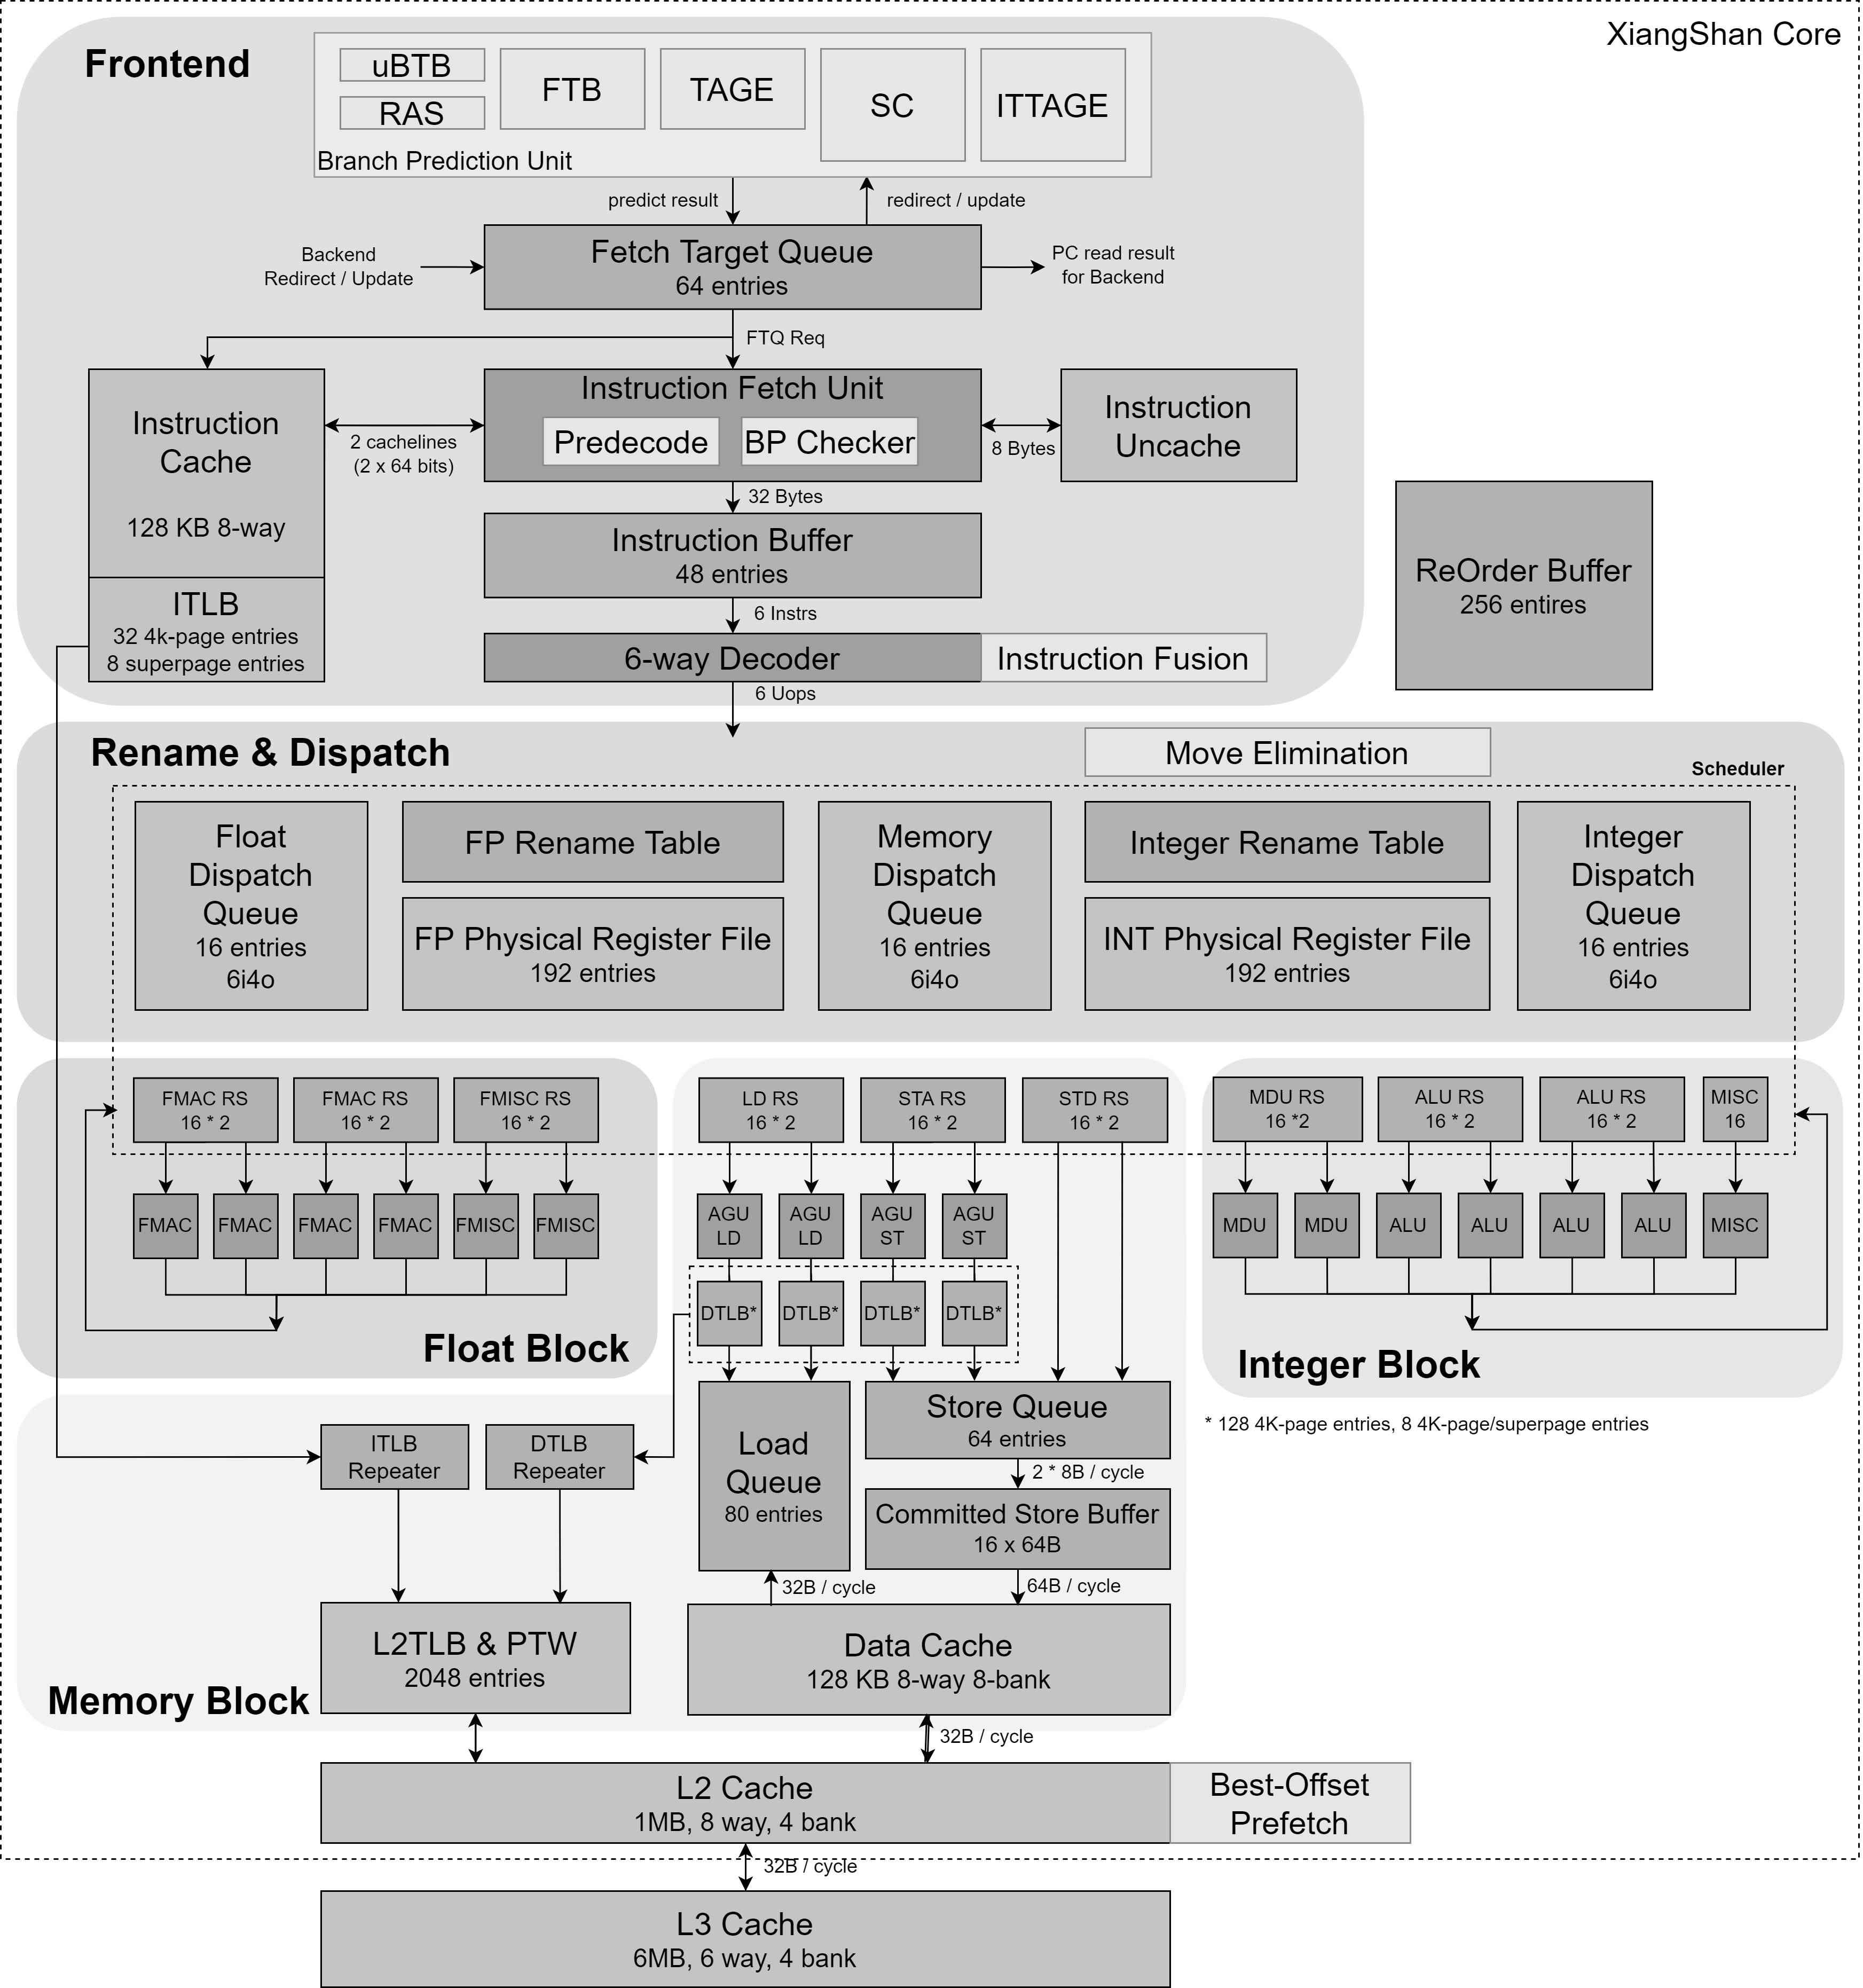
\includegraphics[width=\textwidth]{figs/nanhu.png}
	\caption{南湖微架构\cite{noauthor_openxiangshan/xiangshan:_nodate}}
	\label{fig:nanhu-uarch}
\end{figure}

由于本章展示的攻击方案围绕南湖微架构展开,本小节将对南湖微架构中与攻击方案有关的预测式
执行、乱序执行机制以及存储器子系统的设计作简单的介绍。

\clearpage

\subsection{预测式执行机制}{Speculative Execution Mechanism}
进入南湖微架构执行流水线的每一条指令的地址都是由分支预测单元(Branch Prediction Unit)提供的。
南湖微架构采取了一种分支预测和指令缓存解耦的取指架构,分支预测单元预测接下来的取指地址,
作为取指请求写入一个队列,这个队列将其发往取指单元,用于读取指令高速缓存(Instruction Cache)。

分支预测单元采用一种多级混合预测的架构,其主要组成部分包括:下一行预测器(Next Line Predictor,NLP)
和精确预测器(Accurate Predictor,APD)。其中,NLP是一个小型跳转目标缓冲区(Micro Branch Target Buffer),
用较小的存储开销提供一个无空泡的快速预测流。
APD中运用了TAGE-SC(TAgged GEometric Length Predictor with Statistical Corrector)
算法用来预测分支方向,并设计有取指地址缓冲区(Fetch Target Buffer)和返回地址栈(Return Address Stack)
用以提供跳转地址。
上述部件都将流水线的提交记录作为训练源,以实现根据历史指令流预测未来指令流的功能。

\subsection{乱序执行机制}{Out-of-Order Execution Mechanism}
在指令的发射阶段,南湖微架构使用保留站(Reservation Station)这一结构选择依赖关系已得到
满足的指令送入执行单元,以实现乱序执行。保留站内的主要存储了指令状态、指令和依赖数据。
保留站对指令进行的操作主要有:在发射阶段的入队、选择、读数据和出队等,在写回阶段的监听
以及对等待指令的唤醒等。保留站的主要模块还包括选择逻辑,用来为入队指令分配空闲表项、选择
就绪的指令进行发射。

运用上述硬件结构,可以实现以数据就绪作为指令可以执行的标准,从而指令被执行的顺序可以和
程序指令流中指令出现的顺序不同。

\subsection{存储器子系统}{Memory Subsystem}
香山处理器南湖微架构的存储器子系统可以分为核内和核外两个部分。

位于核内的存储器子系统包括执行单元中的读取、写入地址、写入数据流水线,
读取队列、写入队列和写入缓冲区,与流水线紧耦合的一级数据高速缓存(L1 Data Cache),
以及存储器管理单元(MMU,包括转译后备缓冲器TLB以及页表遍历器TLB)。

位于核外的存储器子系统主要是二级高速缓存(L2 Cache)。这一高速缓存同时具有一致性管理器(Coherence Manager)
的功能,为基于目录的非包含高速缓存(Directory-Based Non-Inclusive Cache),这意味着
在二级高速缓存内维护者一个列表,记录了目前存在于一级高速缓存中的地址(但并不同时存储这些
地址对应的数据),这允许二级高速缓存在外部接口收到一致性维护请求后,通过内部接口通知一级
高速缓存提供最新的数据并将对应缓存行(Cache Line)置为无效状态。


\section{攻击方案}{Attack Plan}
本次攻击将采用Spectre边界检查绕过(Spectre v1 Bounds Check Bypass)\cite{kocher_spectre_2019}方案,
在香山处理器南湖微架构上实现对任意地址的读取。

首先介绍本攻击方案的攻击攻击面(Attack Surface),也就是被攻击的点位。考虑如算法清单\ref{algo:victim}
所示的函数,$a1$是一个长度为$a1\_length$的数组,其中存放着合法的用于索引$a2$数组的下标,
$x$是一个来自外部并且攻击者可控的参数,用来索引$a1$。这样的结构在真实程序中十分常见,一个可能的例子是:$a2$
是一个存储结构体的数组,而$a1$中收集了一些具有特殊性质的结构体位于$a2$中的下标,此时算法清单\ref{algo:victim}
所示的函数就可以被用来访问这些具有特殊性质的结构体。

\begin{algorithm}
	\caption{Victim Function}\label{algo:victim}
	\hspace*{\algorithmicindent} \textbf{Input} $x$ \\
	\hspace*{\algorithmicindent} \textbf{Output} $data$
	\begin{algorithmic}[1]
		\Function{Victim}{}
			\If {$0 \leq x$ \textbf{and} $x < \textit{a1\_length}$} \label{line:guard}
				\State $index \gets \textbf{MEM}[a1 + x]$ \label{line:access-a1}
				\State $offset \gets \text{calculate\_offset}(index)$ \label{line:calc-off}
				\State $data \gets \textbf{MEM}[a2 + offset]$ \label{line:access-a2}
			\Else
				\State $data \gets \text{some invalid value}$
			\EndIf
		\EndFunction
	\end{algorithmic}
\end{algorithm}

可以看到,由于$x$是来自外部的参数,为了安全起见,函数在第\ref{line:guard}行对其进行了边界检查
(Bounds Check),防止在第\ref{line:access-a1}行访问$a1$时越界。紧接着在第\ref{line:calc-off}行,
函数通过从$a1$中的第$x$个位置上取得的索引值,计算要访问的内容在$a2$中的偏移量,对于之前提到的
结构体的实例,calculate\_offset函数可以是简单地将索引值与结构体的大小相乘。在第\ref{line:access-a2}行,
函数使用计算好的偏移量访问$a2$对应的存储器区域。

假设上述函数对不可靠外部参数$x$未做校验就用于索引$a1$,即删去第\ref{line:guard}行的条件判断语句,
攻击者就可以利用第\ref{line:access-a1}行对$a1$的访问实现对任意存储器地址的读取,具体为:假设关注的
地址为$secret$,则可以令$malicious\_x=secret-a1$,并控制传入Victim函数的参数,使$x=malicious\_x$。
这样一来,第\ref{line:access-a1}行就变成了:
\begin{equation}
	\begin{aligned}
		index &\gets \textbf{MEM}[a1 + malicious\_x] \\
		\mbox{即\quad} index &\gets \textbf{MEM}[a1 + (secret - a1)] \notag\\
		\mbox{即\quad} index &\gets \textbf{MEM}[secret]
	\end{aligned}
\end{equation}
\noindent 此时,$index$中存储的即为$secret$地址中的内容。

首先介绍如何实现对第\ref{line:guard}行边界检查的绕过。
边界检查在运行时是以分支指令的形式存在的,现代高性能处理器的预测式执行机制
在分支方向无法及时确定时,会通过考察这一分支指令之前的执行结果,来推测此次的分支方向。如果
连续多次使用合法的$x$作为参数调用Victim函数,“训练(Train)”分支预测器,使其认为这一分支会向合法的
方向跳转,并在使用$x=malicious\_x$作为参数时使得分支指令的条件无法及时确定,就可以使处理
器预测式地使用$malicious\_x$执行访问存储器的指令,从而读取$secret$地址中的内容作为$index$
并继续执行后续的指令。要使边界检查分支指令的条件无法快速确定有很多种手段,最简单的就是确保
在调用Victim函数前,$a1\_length$不存在于高速缓存中,这样会导致在分支条件判断时发生缓存缺失
(Cache Miss),由于上文提到的DRAM延迟较大的问题,就可以实现分支条件的延迟确定。

上述操作可以被称为“误导预测执行流”。
但值得注意的是,即使可以绕过边界检查,将位于$secret$地址的数据读取到$index$中,也要意识到
这些操作及后续执行的指令都是预测式地被执行的,随后一旦边界检查结果被最终确定为越界,上述指令
的执行结果并不会被提交进入体系结构状态,而是会被丢弃,所以这些指令也被称为瞬态指令(Transient
Instructions)。更加确定的是,$index$的值并不会直接返回给调用者,本文接下来讨论如何得到
$index$的值。

虽然瞬态指令的执行结果不会被提交进入体系结构状态,但它们仍然可能对非体结构的状态造成修改。
例如,对于瞬态存储器读取(Load)指令,虽然从存储器子系统读取到的数据不会写入体系结构寄存器
中,但会导致原本不在高速缓存中的被访问的缓存行被换入高速缓存中。读取指令的延时是不确定的,
在高速缓存命中时,请求的数据会很快从就近的高速缓存中返回,此时延时较低;同理当高速缓存缺失
时,请求的数据就需要从上一级高速缓存甚至DRAM中返回,此时延时较高。所以,只要在瞬态读取指令
执行前将瞬态指令可能访问的地址移出高速缓存(Flush),接着执行瞬态读取指令,执行的过程中,某个缓存行
会被重新移入高速缓存(Reload),随后经过探测对感兴趣的地址执行读取指令时所消耗的时间(Time),
就可以精确地确定瞬态读取指令访问的内存地址。这样的操作由\citet{gullasch2011cache}
在2011年首次提出,并被命名为Reload+Time缓存侧信道攻击。

至此,使用Spectre边界检查绕过攻击方案读取位于$secret$地址的数据的操作已经可以完整实现了,
其流程如算法清单\ref{algo:spectre}所示。

\begin{algorithm}
	\caption{Spectre Attack}\label{algo:spectre}
	\begin{algorithmic}[1]
		\Function{Spectre}{}
			\State flush $a2$ out of cache \label{line:flush-a2}
			\Repeat \label{line:train-begin}
				\State call Victim with legal $x$
			\Until{branch predictor is trained} \label{line:train-end}
			\State flush $a1\_length$ out of cache \label{line:flush-a1l}
			\State call Victim with $malicious\_x$ \label{line:call-victim}
			\For{$i \gets \text{possible values of }secret$} \label{line:time-begin}
				\State $result_{i} \gets \text{read\_latency}(\textbf{MEM}[a2 + \text{calculate\_offset}(i)])$
		  	\EndFor \label{line:time-end}
			\State $secret \gets \argmin\limits_{i} result_{i}$ \label{line:find-secret}
		\EndFunction
	\end{algorithmic}
\end{algorithm}

在Spectre攻击方案中,第\ref{line:flush-a2}行将$a2$整个移出高速缓存,为随后的Reload+Time缓存
侧信道攻击恢复$secret$做准备;第\ref{line:train-begin}至\ref{line:train-end}行使用合法的$x$调用
Victim函数,训练分支预测器使其认为$x$大概率处于边界之内;第\ref{line:flush-a1l}行将$a1_length$移出
高速缓存,以制造边界检查分支条件无法很快确定的情形;第\ref{line:call-victim}行使用将会导致处理器
预测式地执行对$secret$地址的读取指令的$malicious\_x$作为参数调用Victim函数,这会导致$a2$中某个与
$secret$地址中的数据值相关的缓存行被换入高速缓存内;第\ref{line:time-begin}至
\ref{line:time-end}行对每个$secret$地址中的数据的可能取值对应的$a2$中的地址进行读取测速,并将
读取所需的时间存储在$result$数组中;最后,第\ref{line:find-secret}行遍历$result$数组,其中访问时间最短
的$i$即最有可能为$secret$地址中的数据的值,至此Spectre攻击方案介绍完毕。

\section{可行性验证}{Feasibility Verification}
为了证明上文中介绍的攻击方案的可行性,接下来将在香山高性能开源RISC-V处理器上实现缓存控制与检测算法与
误导预测执行流算法并最终实现完整的Spectre边界检查绕过攻击。

本文使用的香山处理器代码版本号(Commit ID)为5095522。

\subsection{缓存控制与检测}{Cache Manipulation and Measurement}
缓存控制与检测部分用于缓存侧信道攻击,其中控制主要是指将特定地址从高速缓存中换出(Flush),
检测是指测量对特定地址读取指令所耗费的时间。

控制特定地址从高速缓存中换出有多种方案,例如x86指令集处理器使用单独的clflush指令将指定地址
从整个存储器子系统的各级高速缓存中换出,写回DRAM;SiFive公司的HiFive Unmatched SoC使用一组映射
到存储器地址空间的控制寄存器(Memory Mapped I/O,MMIO)实现相同功能。

\begin{algorithm}
	\caption{Cache Evict}\label{algo:cache-evict}
	\hspace*{\algorithmicindent} \textbf{Input} $address$
	\begin{algorithmic}[1]
		\Function{Evict}{}
			\State $index \gets \text{get\_index}(address)$
			\For{$i \gets \text{ ways of the cache}$}
				\State access $\textbf{MEM}[\text{generate\_tag}(i) + index]$
		  	\EndFor
		\EndFunction
	\end{algorithmic}
\end{algorithm}

香山处理器没有提供从高速缓存中换出特点地址的
直接实现方案。由于从存储器地址空间中的地址到高速缓存行之间是多对一的映射关系,即有多个可能的地址被映射
到同一缓存行。基于这样的特点,可以通过访问与需要被换出的地址映射到相同缓存行的其他地址,将其他地址
换入高速缓存,替换(Evict)掉需要被换出的地址。这种算法涉及到的过程有:计算需要被换出地址对应的
高速缓存索引(Index);生成一组与目标索引一致的候选地址;访问足够多的候选地址,以替换可能存在于
不同高速缓存路(Way)中的目标地址。具体流程如算法\ref{algo:cache-evict}所示。这一算法需要依据
高速缓存的参数实现候选地址的生成,表\ref{tab:cache-param}归纳了香山处理器精简配置的数据缓存参数。

\begin{table}[!ht]
	\centering
\begin{threeparttable}[b]
\zihao{5}
\caption{香山处理器MinimalConfig数据高速缓存参数}
\begin{tabular}{ccccc}
	\toprule
	高速缓存层级 & 缓存行大小(字节) & 缓存行索引数量 & 路数量 & 缓存总大小(字节) \\
	\midrule
	一级 & 64 & 64 & 8 & 32k \\
	二级 & 64 & 1024 & 8 & 512k \\
	\bottomrule
\end{tabular}
\label{tab:cache-param}
\end{threeparttable}
\end{table}

在缓存的检测部分,需要实现对特定地址执行读取指令所耗费的时间的精确测量。RISC-V指令集中,
设计有mcycle控制与状态寄存器(Control and Status Register,CSR),这一寄存器内存储有
处理器自最近一次复位以来已运行的时钟周期数,可作为准确的时间基准。在香山处理器设计中,对
CSR的读写指令会保证与其他指令间的严格顺序(即串行化),意味着乱序执行机制不会对存储器读取
指令时间的测量产生影响。所以只需在存储器读取指令前后各加入一条对mcycle寄存器的读取指令,
分别获得存储器读取前后的处理器时钟周期数,两者之差即为以时钟周期为单位的存储器读取延时。

为了测试上述缓存控制与检测方案的有效性,使用如算法\ref{algo:cache-test}所示的程序
进行测试。结果记录在表\ref{tab:cache-test-result}中。由测试结果可见:缓存控制与检测
方案有效,从一级高速缓存读取的延迟为16个时钟周期,从二级高速缓存读取的延迟为35个时钟周期,
从DRAM读取的延迟为约200至260个时钟周期.

\begin{breakablealgorithm}
	\caption{Timed Read}\label{algo:cache-test}
	\begin{algorithmic}[1]
		\Function{CacheManupulationTest}{}
			\Comment{system cold start, nothing in cache at the beginning}
			\State $address \gets \text{some address in DRAM address range}$
			\State $time1 \gets \text{timed\_read}(address)$
			\State $time2 \gets \text{timed\_read}(address)$
			\State $\text{evict\_l1}(address)$
			\State $time3 \gets \text{timed\_read}(address)$
			\State $\text{evict\_l1}(address)$
			\State $\text{evict\_l2}(address)$
			\State $time4 \gets \text{timed\_read}(address)$
			\State $time5 \gets \text{timed\_read}(address)$
		\EndFunction
	\end{algorithmic}
\end{breakablealgorithm}

\begin{table}[!ht]
	\centering
\begin{threeparttable}[b]
\zihao{5}
\caption{缓存控制与检测方案测试结果}
\begin{tabular}{x{0.2\textwidth}x{0.2\textwidth}}
	\toprule
	结果项 & 结果值 \\
	\midrule
	time1 & 194 \\
	time2 & 16 \\
	time3 & 35 \\
	time4 & 259 \\
	time5 & 16 \\
	\bottomrule
\end{tabular}
\label{tab:cache-test-result}
\end{threeparttable}
\end{table}

\subsection{误导预测执行流}{Misleading Speculative Execution Stream}
为了误导预测执行流,需要先对分支预测器进行训练,即连续多次使用合法参数调用Victim函数。
本攻击实例采用训练5次攻击1次的方案,最简单的实现方案如图\ref{fig:attach-with-branch}
中的C语言代码所示。

\begin{figure}[ht]
	\centering
	\begin{lstlisting}[language=c, escapechar=|]
for (int i = 0; i < 30; i++) {
	if (i % 6 == 0) { |\label{line:related-branch}|
		victim(malicious_x); |\label{line:bad-attack}|
	} else {
		victim(legal_x);
	}
}
	\end{lstlisting}
	\caption{包含条件判断的攻击代码}
	\label{fig:attach-with-branch}
\end{figure}

实验表明上述代码无法正常误导预测执行流,分支预测器会判定第\ref{line:bad-attack}行对Victim
函数的调用参数越界。这是因为分支预测器除了会考量当前分支指令的历史(Local History,局部历史),
也会根据最近执行过的其他分支指令的跳转方向(全局历史,Global History)做出预测。所以分支预测器
正确地推测出了第\ref{line:related-branch}行的分支与边界检查分支有关联。为了解决这个问题,需要
在不使用条件判断分支指令的情况下选择合法的$x$或攻击用的$malicious\_x$作为参数传递给Victim函数。

\begin{figure}[ht]
	\centering
	\begin{lstlisting}[language=c, escapechar=~]
for (int i = 0; i < 30; i++) {
	uint32_t upper_mask = ((i % 6) - 1) & 0xFFFF0000; ~\label{line:gen-upper}~
	uint32_t full_mask = (upper_mask | (upper_mask >> 16)); ~\label{line:gen-full}~
	uint32_t x = legal_x ^ (full_mask & (malicious_x ^ legal_x)); ~\label{line:select-x}~
	victim(x); ~\label{line:call-victim}~
}
	\end{lstlisting}
	\caption{不包含条件判断的攻击代码}
	\label{fig:attach-without-branch}
\end{figure}

图\ref{fig:attach-without-branch}所示的C语言代码实现了相同的功能,但没有额外的分支语句对攻击
指令流造成干扰,其原理如下:第\ref{line:gen-upper}行生成高16位掩码,第\ref{line:gen-full}行生成
完整的32位掩码,第\ref{line:select-x}行使用32位掩码选择legal\_x或malicious\_x作为x的值,
第\ref{line:call-victim}行调用Victim函数。第\ref{line:gen-upper}和\ref{line:gen-full}行
分步生成掩码是因为表达式(i \% 6) - 1在(i \% 6) $\in \{1,2,3,4,5\}$时高16位均为0,但低16位的
部分不能确定,在(i \% 6)为0时高16位均为1,这样可以稳定生成高16位部分的掩码,随后将高16位
复制到低16位区域,即可实现生成完整掩码。这样,在(i \% 6) != 0的训练轮,掩码full\_mask各位均为0,
(full\_mask \& (malicious\_x \^{} legal\_x))也为0,并且由于公式\ref{eq:xor-1}的性质,x取值legal\_x;
在(i \% 6) == 0的攻击轮,掩码full\_mask各位全为1,
(full\_mask \& (malicious\_x \^{} legal\_x))取值(malicious\_x \^{} legal\_x),并且由于公式\ref{eq:xor-2}的性质,
x取值malicious\_x;
表\ref{tab:var-list}列出了两种不同情况下算法中各变量的取值情况。

\begin{equation}
    X \oplus 0 = X \label{eq:xor-1}
\end{equation}
\begin{equation}
	a \oplus X \oplus a = X \label{eq:xor-2}
\end{equation}

\begin{table}
	\centering
\begin{threeparttable}[b]
\zihao{5}
\caption{不包含条件判断的攻击代码变量取值情况}
\begin{tabular}{x{0.2\textwidth}x{0.2\textwidth}x{0.2\textwidth}}
	\toprule
	变量名 & \shortstack{(i \% 6) != 0 \\ 训练轮} & \shortstack{(i \% 6) == 0 \\ 攻击轮} \\
	\midrule
	upper\_mask & 0x0000\_0000 & 0xFFFF\_0000 \\
	full\_mask & 0x0000\_0000 & 0xFFFF\_FFFF \\
	x & legal\_x & malicious\_x \\
	\bottomrule
\end{tabular}
\label{tab:var-list}
\end{threeparttable}
\end{table}

\newpage

\subsection{香山南湖架构攻击验证}{Attack Verification on Nanhu Microarchitecture}
附录\ref{app:spectre-code}中列出了上一小节中介绍的Spectre边界检查绕过攻击方案的C语言实现,阅读代码可以发现
作为攻击目标的模拟秘密数据secret值被设置为了字母G(其ASCII值为71),在整个攻击程序中,
没有任何代码直接读取了secret的值。
编译后,在香山处理器南湖微架构的RTL仿真器上运行这一漏洞利用程序,得到了
如\ref{fig:spectre-result}图所示的结果。

\begin{figure}[ht]
	\centering
	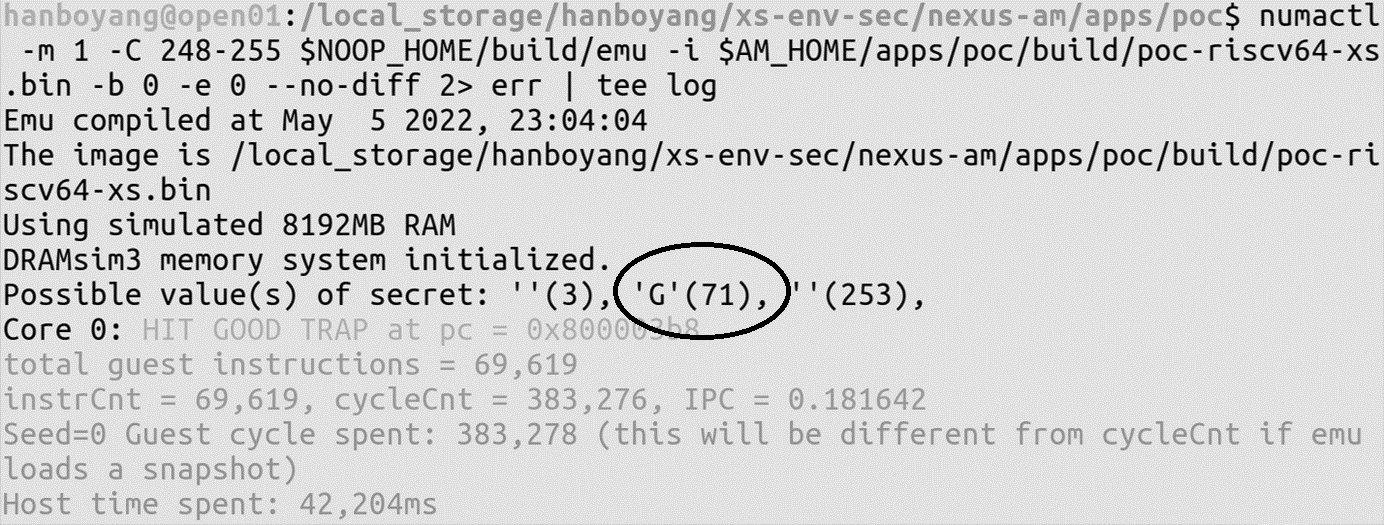
\includegraphics[width=\textwidth]{figs/spectre-result.png}
	\caption{Spectre漏洞利用程序运行结果}
	\label{fig:spectre-result}
\end{figure}

可见程序给出了3个可能的secret值:其中字母G,是secret的值,证明本章
介绍的攻击方案有效;3是用于训练分支预测器使用的参数,在更精密设计的
攻击程序中,可以通过多次执行攻击,轮换分支预测器训练值来降低这类干扰;253出现的原因是
由于高速缓存作为传递秘密信息的侧信道,其信噪比较低导致的,也可以通过多次执行攻击并通过
统计手段滤除此类干扰。


\section{本章小结}{Chapter Summary}
本章首先介绍了现代高性能处理器的设计理念:超标量流水线、乱序执行、预测式执行和存储器子系统
分层高速缓存,以及这些理念产生的背景。

接着介绍了Spectre边界检查绕过攻击方案的整体思路,并详细介绍了利用预测式执行机制绕过边界检查、
使用高速缓存侧信道传递信息的步骤。

最后使用C语言实现了攻击方案,并针对几处需要特别注意的实现细节进行了详细说明。
然后在香山处理器RTL仿真器上证明了攻击方案的可行性,根据测试结果分析了攻击方案的不足,并
针对性地提出了完善思路。


\newpage

% !TeX root = ../thesis.tex

\chapter{针对处理器系统的攻击}{Attacks on Processor Systems}


\section{处理器系统及其通常结构}{Processor Systems and Their Common Structures}
\somewords


\section{SiFive Freedom U740 SoC结构}{Structure of the SiFive Freedom U740 SoC}
\somewords
\subsection{片上互联}{On-Chip Interconnect}
\somewords
\subsection{PCIe 子系统}{PCIe Subsystem}
\somewords


\section{基于DMA的攻击}{DMA-Based Attack}
\somewords


\section{PCIe DMA攻击实例}{An Attack Example Based on PCIe DMA}
\somewords
\subsection{PCIe Endpoint实现}{Implementation of PCIe Endpoint}
\somewords
\subsection{Linux 物理地址获取}{Acquisition of Physical Address on Linux}
\somewords
\subsection{秘密信息读取}{Readout of Secret Data}
\somewords

\section{本章小结}{Chapter Summary}
\somewords


\newpage

% !TeX root = ../thesis.tex

\chapter{总结与展望}{Conclusion and Outlook}



\newpage

\nocite{*} 
\bibliography{ref}
\appendix
\chapter{Spectre漏洞利用代码}{Spectre Proof-of-Concept Code} \label{app:spectre-code}
\lstinputlisting[language=c]{body/spectre.c}

\chapter{虚拟到物理内存地址翻译程序}{Virtual to Physical Address Translator} \label{app:v2p}
\lstinputlisting[language=c]{body/v2p.c}

\chapter{PCIe设计框图}{Block Design of PCIe Endpoint} \label{app:pcie-ep}
\begin{sidewaysfigure}
	\centering
	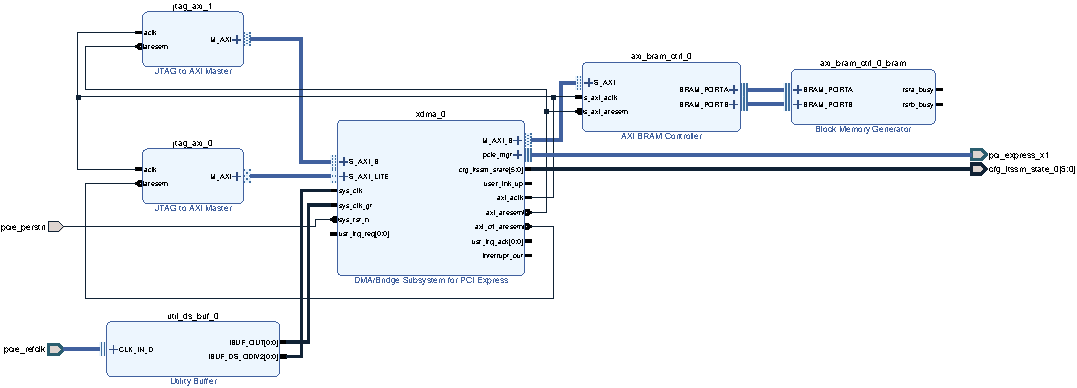
\includegraphics[width=\textwidth]{figs/pcie-ep.pdf}
	\caption{软件可控PCIe Endpoint Block Design}
\end{sidewaysfigure}
% \backmatter
% 后记
\end{document}
